\documentclass[12pt,a4paper]{article}

\usepackage[T1]{fontenc}
\usepackage[utf8]{inputenc}
\usepackage[brazil]{babel}
\usepackage{lmodern}
\usepackage[a4paper,margin=2.5cm]{geometry}
\usepackage{graphicx}
\usepackage{booktabs}
\usepackage{longtable}
\usepackage{float}
\usepackage{amsmath}
\usepackage{hyperref}
\usepackage{xcolor}
\usepackage{enumitem}

\hypersetup{colorlinks=true,linkcolor=blue!50!black,urlcolor=blue!50!black,citecolor=blue!50!black}

\title{Avaliação de representações contínua e simbólica de sinais de ECG com LSTM: uma análise por escalas temporais}
\author{Tiago Leite Pereira}
\date{2026}

\begin{document}

\maketitle

\begin{abstract}
Este trabalho avalia o efeito da redução temporal e da simbolização na classificação automática de batimentos cardíacos a partir de sinais de eletrocardiograma. Foram utilizados 46 registros da MIT-BIH Arrhythmia Database, totalizando 105.036 batimentos anotados. Cada batimento foi representado por uma janela de 250 amostras, normalizada individualmente e submetida a coarse-graining por médias em blocos de $t$ amostras, com $t$ variando de 2 a 10. Para cada escala foram comparadas duas entradas para uma rede LSTM: uma representação contínua, formada pelas médias dos blocos, e uma representação simbólica, obtida pela discretização dessas médias em um alfabeto de sete símbolos. A tarefa supervisionada foi a detecção binária de batimentos não normais, agrupando as classes AAMI $S$, $V$, $F$ e $Q$. A avaliação utilizou cinco divisões estratificadas por registro, com limiar ajustado na validação. A configuração simbólica com $t=5$ apresentou o melhor equilíbrio médio, com balanced accuracy de 0,866, sensibilidade de 0,767 e especificidade de 0,966. Os resultados indicam que a simbolização pode reduzir a representação temporal mantendo desempenho competitivo, embora o compromisso entre falsos positivos e falsos negativos dependa da escala escolhida.
\end{abstract}

\noindent\textbf{Palavras-chave:} eletrocardiograma; dinâmica simbólica; coarse-graining; LSTM; arritmia; aprendizado de máquina.

\section{Fundamentação teórica}

\subsection{Representação simbólica de séries temporais}

Uma série temporal contínua pode ser transformada em uma sequência simbólica por meio de uma partição do espaço de amplitudes. Seja $x_i$ a amplitude na posição temporal $i$ e seja $\{b_0,b_1,\ldots,b_K\}$ o conjunto de limites da partição. A função simbólica é definida por

\begin{equation}
    s_i = k \quad \text{se} \quad b_k \leq x_i < b_{k+1},
\end{equation}

com $s_i \in \{0,1,\ldots,K-1\}$. A sequência resultante mantém o índice temporal da observação, mas reduz a resolução da amplitude. A informação dinâmica é analisada por meio de transições, palavras simbólicas, distribuição de frequências e entropia.

Essa distinção é importante para o presente estudo. A simbolização ponto a ponto não reduz necessariamente o número de amostras. A redução temporal ocorre em uma etapa separada, o coarse-graining, realizado antes da aplicação da partição simbólica.

\subsection{Simbolização por pico e simbolização morfológica}

A estratégia desenvolvida anteriormente pelo autor utiliza os picos cardíacos como eventos de referência. Nessa formulação, cada batimento contribui com um valor, como a amplitude do pico ou um intervalo entre picos, e a sequência representa a evolução entre batimentos. Seu comprimento é, portanto, aproximadamente igual ao número de batimentos do registro.

Na estratégia analisada neste artigo, cada batimento é tratado como uma trajetória morfológica. Uma janela de 250 amostras é transformada em uma sequência de amplitudes agregadas e, posteriormente, em uma sequência simbólica. A sequência representa a evolução interna do batimento, incluindo regiões associadas às ondas P, ao complexo QRS e à onda T. As duas estratégias não devem ser interpretadas como substitutas diretas: a primeira descreve dinâmica entre eventos e a segunda descreve morfologia dentro do evento.

\subsection{Coarse-graining multiescala}

O coarse-graining temporal é utilizado em análises multiescala de sinais fisiológicos para produzir representações em diferentes resoluções. Neste trabalho, a escala $t$ possui interpretação direta: cada observação agregada corresponde à média de $t$ amostras consecutivas do ECG normalizado. Escalas menores preservam mais detalhes locais; escalas maiores produzem sequências mais curtas e potencialmente mais robustas a pequenas oscilações.

Essa escolha cria uma hipótese experimental verificável: deve existir uma faixa intermediária na qual a redução de ruído e de dimensionalidade compense a perda de detalhes morfológicos. A varredura de $t=2$ a $t=10$ foi construída para testar essa hipótese, e não para assumir previamente que uma escala específica seria ótima.

\subsection{Interpretação da escala $t$}

Neste artigo, $t$ não representa o número de símbolos do alfabeto. Ele representa o número de amostras originais reunidas em cada bloco temporal. Portanto, há duas operações conceitualmente distintas: primeiro, a média reduz a resolução no eixo temporal; depois, a partição reduz a resolução no eixo de amplitude. Essa distinção evita interpretar a sequência simbólica como uma simples redução do número de pontos do sinal.

Como a frequência de amostragem é de 360 Hz, cada amostra corresponde a aproximadamente 2,78 ms. Assim, $t=2$ corresponde a blocos de aproximadamente 5,56 ms, enquanto $t=10$ corresponde a blocos de aproximadamente 27,78 ms. A janela de 250 amostras cobre aproximadamente 694,4 ms. A tabela abaixo mostra o efeito direto da escala sobre o comprimento da entrada da rede.

\begin{table}[H]
\centering
\caption{Relação entre a escala temporal, a duração do bloco e o tamanho da sequência.}
\label{tab:escalas_temporais}
\small
\begin{tabular}{rrrr}
\toprule
$t$ & Amostras/bloco & Duração aproximada (ms) & $L_t$ \\
\midrule
2 & 2 & 5,56 & 125 \\
3 & 3 & 8,33 & 83 \\
4 & 4 & 11,11 & 62 \\
5 & 5 & 13,89 & 50 \\
6 & 6 & 16,67 & 41 \\
7 & 7 & 19,44 & 35 \\
8 & 8 & 22,22 & 31 \\
9 & 9 & 25,00 & 27 \\
10 & 10 & 27,78 & 25 \\
\bottomrule
\end{tabular}
\end{table}

Por exemplo, em $t=5$, cada conjunto de cinco amostras é substituído por uma única média. A janela original passa de 250 valores contínuos para 50 valores contínuos. Na entrada simbólica, esses 50 valores são ainda convertidos em 50 índices pertencentes ao alfabeto. Portanto, a rede recebe 50 posições temporais tanto no modelo contínuo quanto no simbólico; o que muda é a codificação do valor em cada posição.

\section{Introdução}

O eletrocardiograma (ECG) é um instrumento central para a avaliação da atividade elétrica cardíaca. A classificação automática de batimentos pode auxiliar a triagem de registros extensos, mas apresenta dificuldades associadas à variabilidade morfológica, ao desbalanceamento entre classes e às diferenças entre pacientes.

Uma alternativa para reduzir a complexidade da representação consiste em substituir valores contínuos por símbolos definidos por uma partição do espaço de amplitudes. Na dinâmica simbólica, essa transformação preserva a ordem temporal e reduz a resolução do espaço de estados. A estratégia desenvolvida na tese de Pereira utiliza uma simbolização orientada por picos, produzindo uma sequência de eventos cardíacos. Neste trabalho, investigamos uma representação complementar: a simbolização ponto a ponto da morfologia de cada batimento.

O objetivo foi comparar uma entrada contínua e uma entrada simbólica para uma LSTM, após redução temporal por médias em blocos. A pergunta experimental foi: qual escala temporal produz o melhor compromisso entre detecção de batimentos não normais e geração de falsos alarmes?

\section{Materiais e métodos}

\subsection{Base de dados e preparação}

Foi utilizada a MIT-BIH Arrhythmia Database. O pipeline considerou 46 registros com sinais filtrados e anotações de batimentos, amostrados a 360 Hz. As anotações originais foram mapeadas para as classes AAMI. O conjunto resultante continha 90.330 batimentos $N$, 7.229 $V$, 3.894 $Q$, 2.781 $S$ e 802 $F$.

Para cada anotação foi extraída uma janela de 250 amostras, com 100 amostras antes e 150 depois da posição anotada. Batimentos cuja janela ultrapassava os limites do registro foram excluídos.

\subsection{Coarse-graining temporal}

Cada janela foi normalizada individualmente por min--max. Em seguida, para cada escala $t \in \{2,3,\ldots,10\}$, a janela foi dividida em blocos não sobrepostos de $t$ amostras. A média de cada bloco produziu uma sequência contínua de tamanho:

\begin{equation}
L_t = \left\lfloor \frac{250}{t} \right\rfloor.
\end{equation}

Quando 250 não era divisível por $t$, as amostras restantes no final da janela foram descartadas. Assim, por exemplo, $t=2$ produziu 125 valores, $t=5$ produziu 50 valores e $t=10$ produziu 25 valores.

\subsection{Representações comparadas}

Foram avaliadas duas representações com o mesmo comprimento $L_t$:

\begin{enumerate}
    \item \textbf{contínua}: médias dos blocos usadas diretamente como entrada da LSTM;
    \item \textbf{simbólica}: médias dos blocos discretizadas em um alfabeto de sete símbolos.
\end{enumerate}

Na representação simbólica, os limites da partição foram calculados exclusivamente com as amostras do conjunto de treinamento de cada divisão. A quantidade de símbolos foi selecionada pelo critério de saturação da variação da entropia. Os mesmos limites foram aplicados à validação e ao teste.

\subsection{Construção do alfabeto simbólico}

O alfabeto foi definido a partir da distribuição empírica das amplitudes agregadas do conjunto de treinamento. Para cada candidato $K$ entre 2 e 16 símbolos, foram calculados limites de partição por quantis de probabilidade. Em seguida, a sequência de valores foi convertida em símbolos e sua entropia de Shannon foi calculada por

\begin{equation}
H_K=-\sum_{j=0}^{K-1}p_j\log_2(p_j),
\end{equation}

em que $p_j$ é a frequência relativa do símbolo $j$. A variação entre dois alfabetos consecutivos foi definida por $\\Delta H_K=H_K-H_{K-1}$. O primeiro ponto em que $\\Delta H_K<0,2$ foi considerado uma saturação; o alfabeto imediatamente anterior foi escolhido. Caso a saturação não ocorresse, seria utilizado o limite máximo de 16 símbolos.

No experimento final, o procedimento selecionou sete símbolos em todas as escalas e repetições. Assim, o número sete não foi imposto manualmente como uma preferência visual: ele foi o resultado do critério de entropia aplicado ao treinamento. Essa informação é relevante para a reprodutibilidade, pois o parâmetro $t$ controla o eixo temporal, enquanto $K=7$ descreve a resolução no eixo de amplitude.

O símbolo não possui, por si só, significado clínico fixo. O índice 0 não significa necessariamente ``normal'' e o índice 6 não significa necessariamente ``patológico''. Cada símbolo apenas identifica um intervalo de amplitude normalizada. O significado discriminativo emerge da sequência e da posição temporal dos símbolos dentro da janela.

\subsection{Tarefa de classificação}

A tarefa principal foi binária:

\begin{equation}
N \rightarrow \text{normal}, \qquad S,V,F,Q \rightarrow \text{não-N}.
\end{equation}

Essa formulação foi escolhida para evitar que a classe majoritária $N$ dominasse a acurácia e para priorizar a identificação de batimentos potencialmente anormais. A classificação não deve ser interpretada como diagnóstico clínico individual.

\subsection{Visualização da transformação}

A Figura~\ref{fig:processo} ilustra o efeito da escala sobre dois batimentos, um normal e um ventricular. A curva preta corresponde às médias dos blocos e os pontos coloridos correspondem aos símbolos, apresentados em uma escala vertical apenas para facilitar a comparação visual. Com $t=2$, a entrada ainda possui 125 posições e acompanha oscilações mais locais. Com $t=5$, restam 50 posições, produzindo uma descrição intermediária. Com $t=10$, restam 25 posições e a sequência enfatiza a forma global do batimento. A figura não altera o treinamento; ela é uma representação didática do mesmo procedimento aplicado a todas as janelas.

\begin{figure}[H]
    \centering
    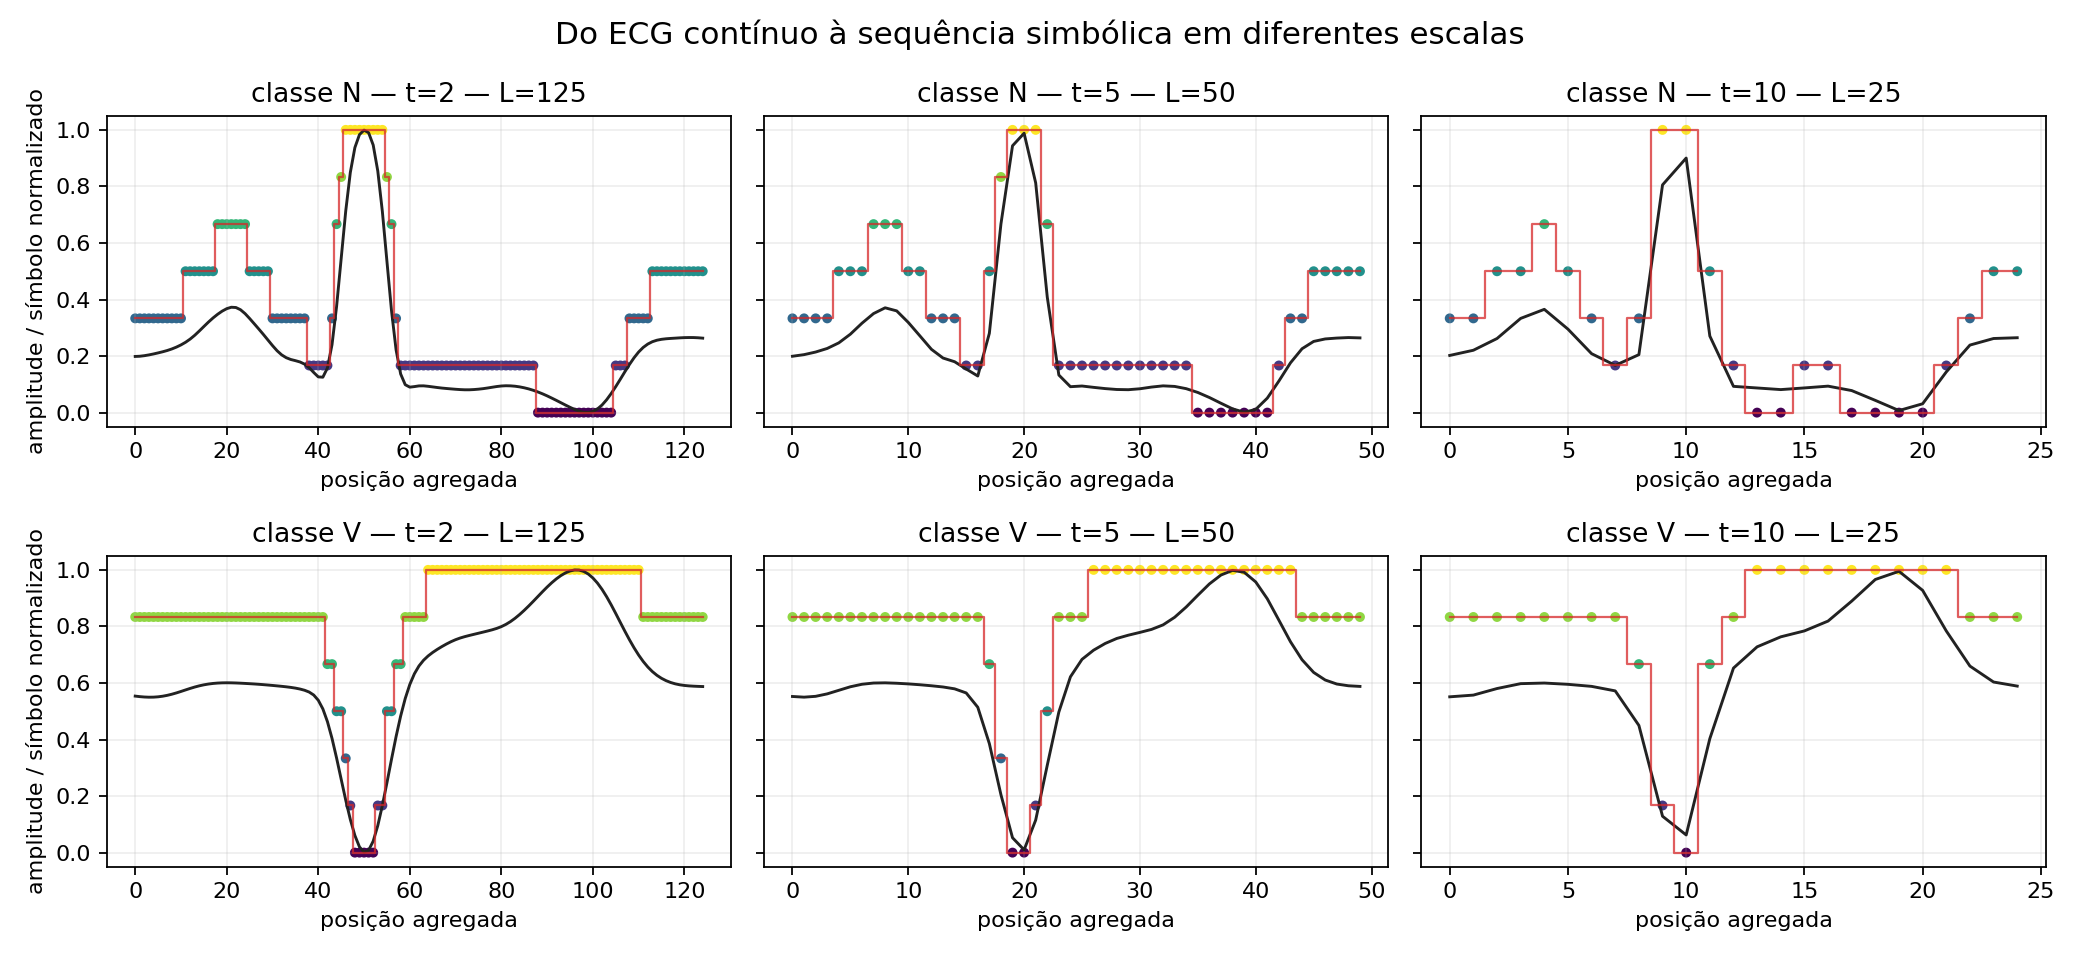
\includegraphics[width=\textwidth]{../symbolic_lstm_scale_sweep_binary_test/scale_process_examples.png}
    \caption{Exemplo do processo de coarse-graining e simbolização para um batimento normal e um batimento ventricular nas escalas $t=2$, $t=5$ e $t=10$.}
    \label{fig:processo}
\end{figure}

\subsection{Modelos e validação}

Foram treinadas redes LSTM com duas camadas recorrentes, dropout e uma camada densa final com ativação sigmoidal. A rede contínua recebeu sequências de valores reais; a rede simbólica recebeu índices inteiros codificados em one-hot antes das camadas LSTM. O treinamento utilizou ponderação de classes e parada antecipada baseada na perda de validação.

Para evitar vazamento entre batimentos do mesmo registro, as divisões foram realizadas por registro usando estratificação agrupada. Foram utilizadas cinco repetições, com sementes 42 a 46, mantendo as mesmas divisões para os modelos contínuo e simbólico em cada repetição. O limiar de decisão foi escolhido na validação maximizando o escore F2, priorizando recall da classe não-N.

As divisões foram mantidas fixas entre escalas. Essa decisão permite atribuir diferenças de desempenho à representação e à escala, em vez de introduzir simultaneamente uma mudança na composição dos pacientes. Para cada repetição, os registros foram separados em conjuntos de treinamento, validação e teste. Nenhum batimento do mesmo registro foi compartilhado entre esses conjuntos.

As métricas principais foram:

\begin{itemize}
    \item verdadeiros positivos (TP), verdadeiros negativos (TN), falsos positivos (FP) e falsos negativos (FN);
    \item sensibilidade de não-N;
    \item taxa de falso negativo;
    \item especificidade de N;
    \item taxa de falso positivo;
    \item balanced accuracy, calculada como a média entre sensibilidade e especificidade.
\end{itemize}

\subsection{Protocolo experimental completo}

O experimento foi organizado para que a comparação entre as representações fosse pareada. Primeiro, os batimentos foram extraídos dos registros e associados ao identificador do registro de origem. Em seguida, cada batimento foi normalizado e submetido a todas as nove escalas temporais. Para uma dada repetição, a mesma lista de registros de treinamento, validação e teste foi reutilizada em todos os valores de $t$ e nos dois modelos. Dessa forma, cada ponto dos gráficos representa uma mudança controlada na representação, e não uma nova amostra aleatória do banco.

Para cada combinação entre repetição e escala, foram executadas as seguintes etapas: (i) aplicar o coarse-graining às 250 amostras de cada janela; (ii) separar os exemplos conforme os índices de registro já definidos; (iii) estimar o alfabeto simbólico somente no conjunto de treinamento; (iv) aplicar a mesma partição às três partes; (v) treinar a LSTM contínua e a LSTM simbólica; (vi) escolher o limiar usando a validação; e (vii) calcular a matriz de confusão e as métricas no teste. A partição simbólica é, portanto, recalculada em cada repetição e escala, mas nunca utiliza amostras de validação ou teste para definir seus limites.

O treinamento dos dois modelos utiliza a mesma arquitetura recorrente: uma LSTM com 32 unidades e retorno da sequência, dropout de 0,3, uma segunda LSTM com 16 unidades, novo dropout, camada densa de 16 unidades com ativação ReLU e saída sigmoidal. No modelo contínuo, cada passo possui um valor real; no simbólico, cada índice é convertido para codificação one-hot com sete componentes. Essa escolha permite comparar a natureza da entrada mantendo constante a capacidade aproximada do classificador.

O desbalanceamento foi tratado com pesos de classe calculados somente a partir do treinamento. A função de perda foi entropia cruzada binária. O treinamento foi limitado a dez épocas, com parada antecipada quando a perda de validação deixou de melhorar por cinco épocas. O limiar não foi fixado automaticamente em 0,5: foram testados 181 valores entre 0,05 e 0,95 na validação, selecionando-se aquele que maximizou o F2. No teste, esse limiar ficou congelado, evitando que a informação do conjunto de avaliação alterasse a decisão.

As quantidades apresentadas nos gráficos são médias das cinco repetições. O desvio-padrão representa a variação entre as divisões por registro, e não a variação entre batimentos dentro de uma mesma divisão. Essa distinção é importante: um desvio-padrão elevado de FP sugere que alguns conjuntos de registros são particularmente difíceis, enquanto não permite concluir, sozinho, que o classificador seja instável em cada batimento individual.

\subsection{Implementação computacional}

O pipeline foi implementado em Python, utilizando NumPy e pandas para manipulação dos dados, scikit-learn para a divisão estratificada por grupos e cálculo das métricas, e TensorFlow/Keras para as redes LSTM. A implementação foi organizada em scripts reprodutíveis. Os limites simbólicos, históricos de entropia, divisões por registro e métricas por repetição foram persistidos em arquivos CSV e JSON.

Para cada escala, o procedimento computacional seguiu a ordem abaixo:

\begin{enumerate}
    \item carregar as janelas anotadas dos 46 registros;
    \item normalizar cada janela individualmente;
    \item calcular a quantidade de blocos completos e descartar o restante;
    \item calcular a média em cada bloco;
    \item construir a entrada contínua;
    \item estimar a partição simbólica apenas no treino;
    \item construir as entradas simbólicas de treino, validação e teste;
    \item treinar os dois modelos com a mesma divisão;
    \item ajustar o limiar na validação e calcular as métricas no teste.
\end{enumerate}

Esse registro explícito das etapas é necessário porque uma partição calculada usando o conjunto completo poderia introduzir informação do teste no treinamento, mesmo que os rótulos não fossem utilizados.

\section{Resultados}

Cada divisão de teste continha 13.599 batimentos, dos quais 1.583 eram não-N. A Figura~\ref{fig:escalas} mostra a variação das principais métricas em função da escala temporal.

\begin{figure}[H]
    \centering
    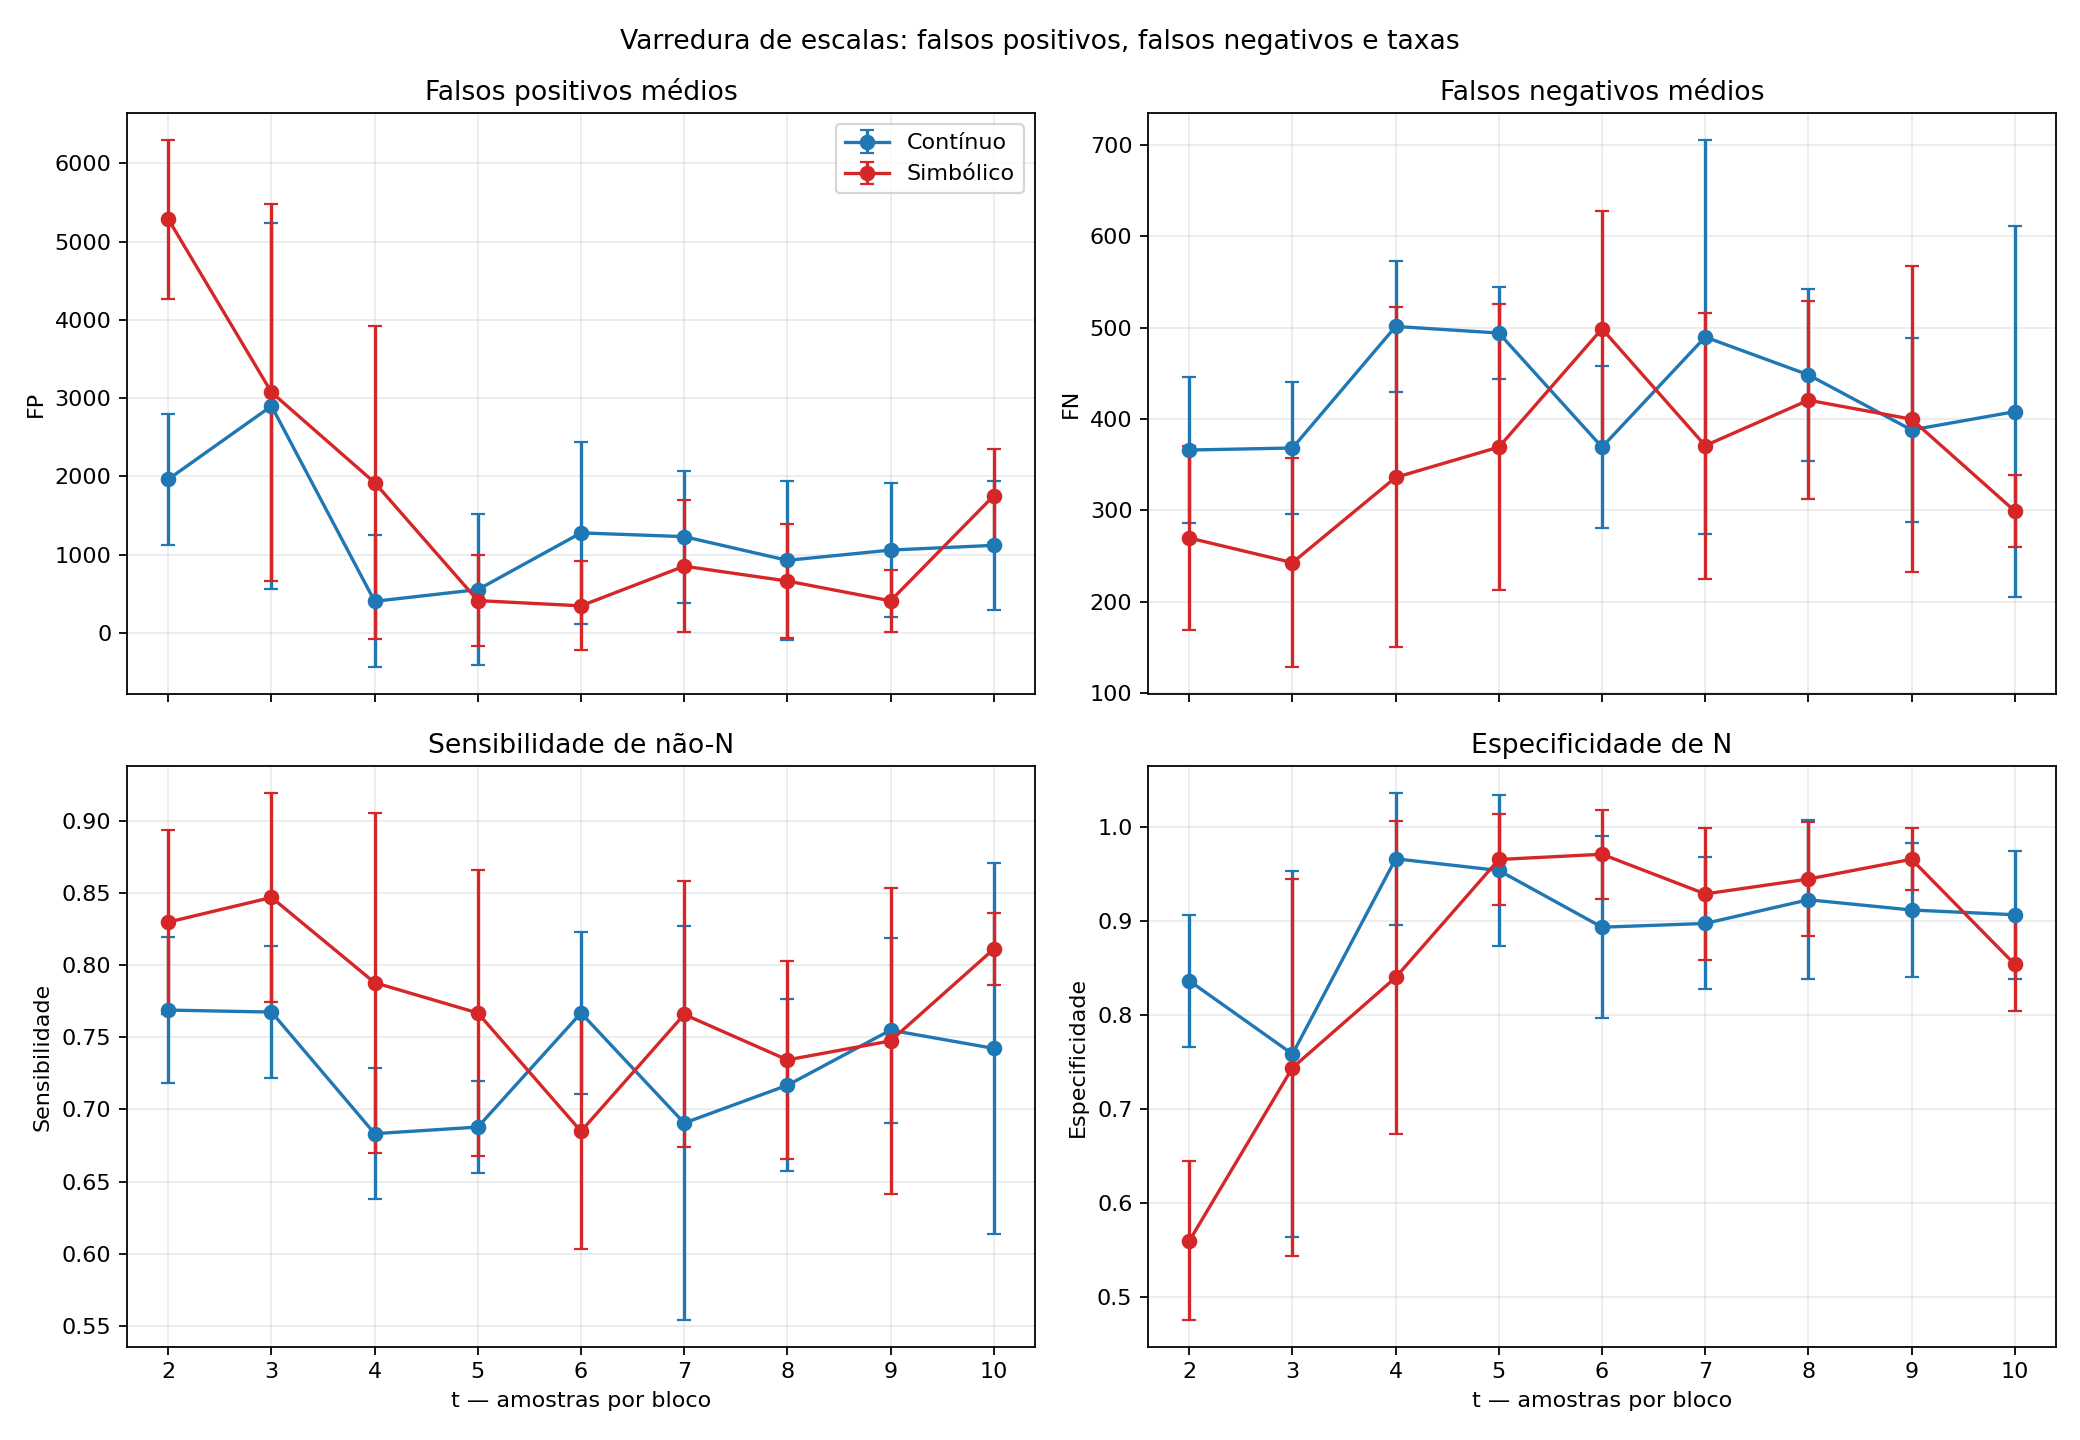
\includegraphics[width=\textwidth]{../symbolic_lstm_scale_sweep_binary_test/scale_sweep_fp_fn_rates.png}
    \caption{Médias e desvios-padrão de falsos positivos, falsos negativos, sensibilidade e especificidade nas cinco repetições.}
    \label{fig:escalas}
\end{figure}

\begin{table}[H]
\centering
\caption{Resultados médios da varredura de escalas.}
\label{tab:resultados}
\scriptsize
\begin{tabular}{ccrrrrrr}
\toprule
Modelo & $t$ & FP & FN & Sens. & Espec. & Bal. acc. & ROC-AUC \\
\midrule
Contínuo & 2 & 1964 & 366 & 0,769 & 0,837 & 0,803 & 0,849 \\
Simbólico & 2 & 5287 & 270 & 0,830 & 0,560 & 0,695 & 0,831 \\
Contínuo & 3 & 2899 & 368 & 0,767 & 0,759 & 0,763 & 0,825 \\
Simbólico & 3 & 3074 & 243 & 0,847 & 0,744 & 0,795 & 0,903 \\
Contínuo & 4 & 405 & 501 & 0,683 & 0,966 & 0,825 & 0,881 \\
Simbólico & 4 & 1920 & 336 & 0,788 & 0,840 & 0,814 & 0,899 \\
Contínuo & 5 & 554 & 494 & 0,688 & 0,954 & 0,821 & 0,917 \\
Simbólico & 5 & 413 & 369 & 0,767 & 0,966 & 0,866 & 0,931 \\
Contínuo & 6 & 1279 & 369 & 0,767 & 0,894 & 0,830 & 0,922 \\
Simbólico & 6 & 346 & 499 & 0,685 & 0,971 & 0,828 & 0,927 \\
Contínuo & 7 & 1231 & 490 & 0,691 & 0,898 & 0,794 & 0,891 \\
Simbólico & 7 & 853 & 371 & 0,766 & 0,929 & 0,847 & 0,930 \\
Contínuo & 8 & 928 & 448 & 0,717 & 0,923 & 0,820 & 0,916 \\
Simbólico & 8 & 663 & 421 & 0,734 & 0,945 & 0,840 & 0,921 \\
Contínuo & 9 & 1059 & 388 & 0,755 & 0,912 & 0,833 & 0,927 \\
Simbólico & 9 & 410 & 400 & 0,747 & 0,966 & 0,857 & 0,935 \\
Contínuo & 10 & 1119 & 408 & 0,742 & 0,907 & 0,825 & 0,921 \\
Simbólico & 10 & 1753 & 299 & 0,811 & 0,854 & 0,833 & 0,923 \\
\bottomrule
\end{tabular}
\end{table}

A melhor balanced accuracy média foi obtida pela representação simbólica com $t=5$, alcançando 0,866. Essa configuração apresentou 413 falsos positivos médios e 369 falsos negativos médios, com sensibilidade de 0,767 e especificidade de 0,966.

A menor quantidade média de falsos negativos foi observada na representação simbólica com $t=3$, com aproximadamente 243 casos. Entretanto, essa configuração produziu cerca de 3.074 falsos positivos médios. A configuração simbólica com $t=6$ apresentou o menor número médio de falsos positivos, aproximadamente 346, mas com aumento dos falsos negativos para aproximadamente 499.

\subsection{Variabilidade entre as repetições}

As médias agregadas não devem ser interpretadas sem considerar a variabilidade entre divisões. A Tabela~\ref{tab:variabilidade} resume os resultados das configurações de referência $t=4$, $t=5$ e $t=6$. Observa-se que a configuração simbólica com $t=5$ apresentou o melhor equilíbrio, mas seu desvio-padrão de falsos positivos ainda é relevante. Isso indica que determinados grupos de registros são mais difíceis de classificar e que a composição do teste influencia o número de alarmes.

\begin{table}[H]
\centering
\caption{Média e desvio-padrão para escalas próximas da configuração selecionada.}
\label{tab:variabilidade}
\small
\begin{tabular}{llrrrr}
\toprule
Modelo & $t$ & FP média & DP(FP) & FN média & DP(FN) \\
\midrule
Contínuo & 4 & 405 & 845 & 501 & 71 \\
Simbólico & 4 & 1920 & 1996 & 336 & 186 \\
Contínuo & 5 & 554 & 964 & 494 & 50 \\
Simbólico & 5 & 413 & 585 & 369 & 157 \\
Contínuo & 6 & 1279 & 1160 & 369 & 89 \\
Simbólico & 6 & 346 & 567 & 499 & 129 \\
\bottomrule
\end{tabular}
\end{table}

\subsection{Compromisso entre falsos positivos e falsos negativos}

A Figura~\ref{fig:fpfn} apresenta o compromisso entre falsos positivos e falsos negativos para todas as escalas. Cada ponto representa a média de cinco repetições e as barras indicam o desvio-padrão. A região ideal depende da finalidade do sistema: deslocar-se para baixo reduz batimentos anormais perdidos, enquanto deslocar-se para a esquerda reduz alarmes falsos.

\begin{figure}[H]
    \centering
    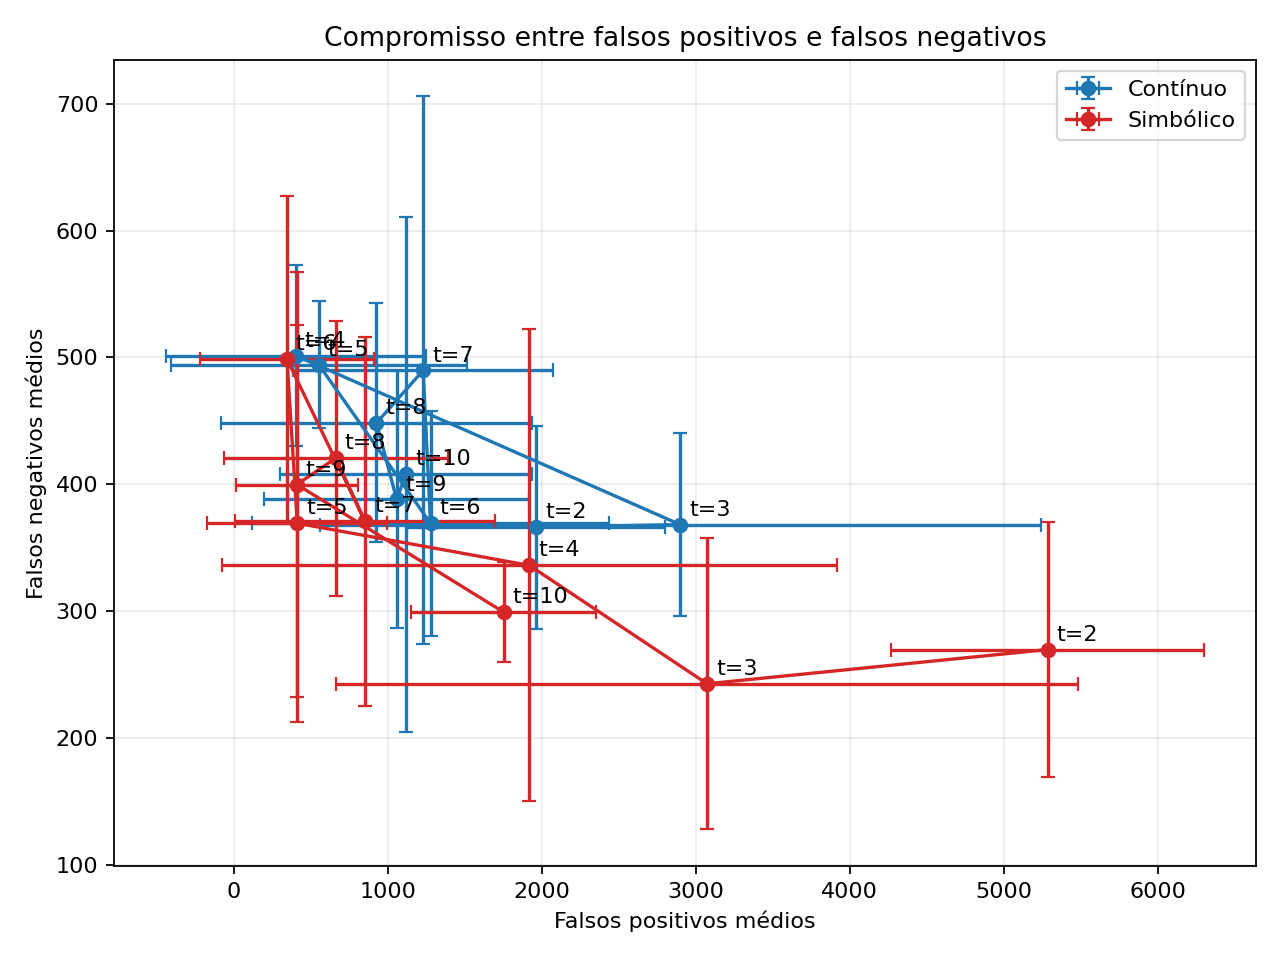
\includegraphics[width=0.82\textwidth]{../symbolic_lstm_scale_sweep_binary_test/scale_sweep_fp_vs_fn.png}
    \caption{Compromisso entre falsos positivos e falsos negativos nas diferentes escalas.}
    \label{fig:fpfn}
\end{figure}

\subsection{Qualidade global por escala}

Embora FP e FN sejam essenciais para a interpretação em saúde, a balanced accuracy oferece uma síntese útil quando as classes são desbalanceadas. A Figura~\ref{fig:balanced} mostra essa métrica para as duas representações. A rede simbólica supera a contínua em várias escalas, com maior diferença em $t=5$, $t=7$ e $t=9$. Essa vantagem não é uniforme: em $t=2$ a representação contínua apresenta desempenho global superior, enquanto em $t=3$ a diferença é pequena.

\begin{figure}[H]
    \centering
    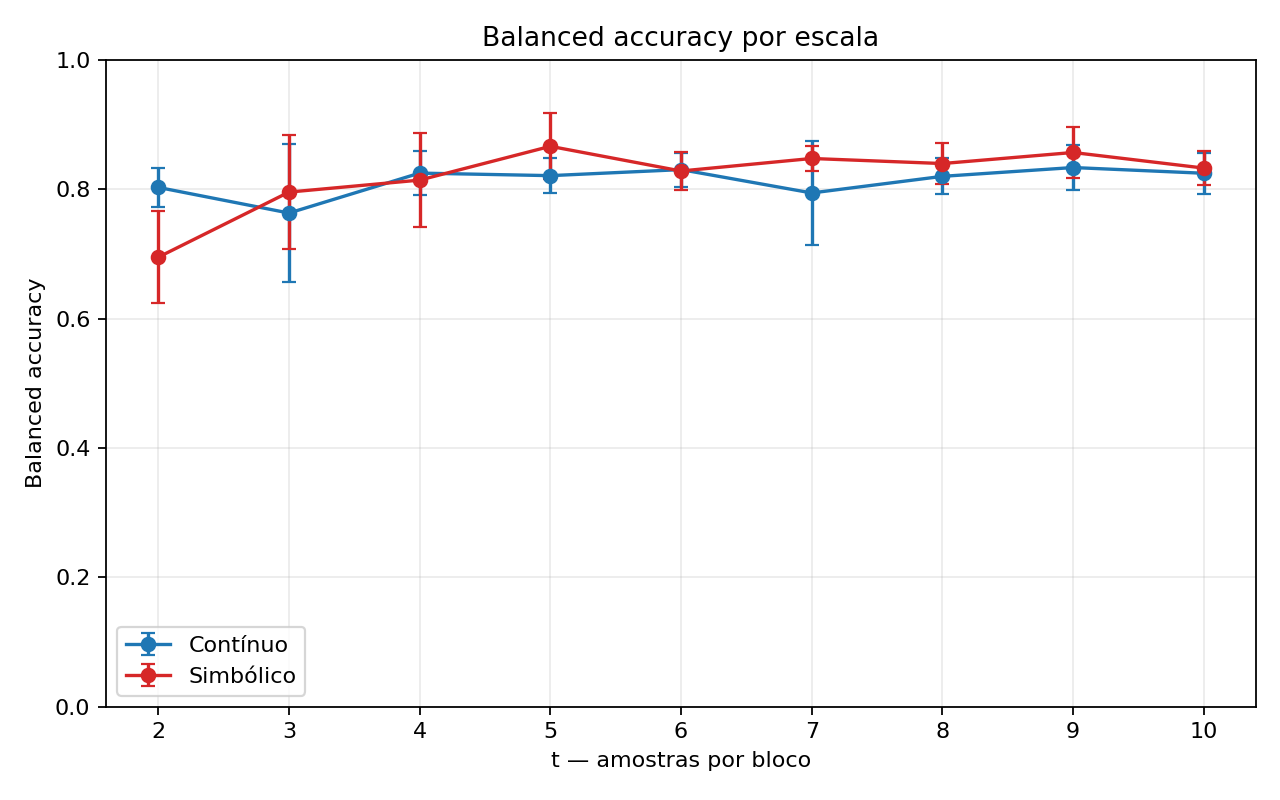
\includegraphics[width=0.82\textwidth]{../symbolic_lstm_scale_sweep_binary_test/scale_sweep_balanced_accuracy.png}
    \caption{Balanced accuracy média e desvio-padrão por escala.}
    \label{fig:balanced}
\end{figure}

\section{Discussão}

Os resultados mostram que a escolha da escala temporal altera diretamente o compromisso entre detecção de batimentos não normais e alarmes falsos. A escala $t=2$ manteve uma sequência mais longa, mas a representação simbólica apresentou baixa especificidade e grande quantidade de falsos positivos. Em escalas intermediárias, especialmente $t=5$ e $t=9$, a representação simbólica apresentou melhor equilíbrio entre sensibilidade e especificidade.

A configuração simbólica com $t=5$ é particularmente interessante porque reduz a janela de 250 amostras para 50 símbolos, preservando uma representação temporal compacta e obtendo a maior balanced accuracy média. O resultado sugere que a redução de resolução pode remover variações locais pouco úteis, enquanto a simbolização mantém padrões qualitativos da morfologia do batimento.

A comparação também evidencia que não existe uma escala ótima independente do objetivo. Se a prioridade for minimizar falsos negativos, $t=3$ simbólico é mais favorável. Se a prioridade for reduzir falsos positivos, $t=6$ simbólico ou $t=4$ contínuo são alternativas mais conservadoras. Em uma aplicação de triagem, a escolha final deve ser associada ao custo relativo de cada tipo de erro.

Os resultados devem ser interpretados com algumas limitações. Primeiro, todos os experimentos foram conduzidos na mesma base MIT-BIH. Segundo, foram utilizadas cinco repetições por registro, o que fornece uma estimativa inicial de variabilidade, mas não substitui validação externa. Terceiro, o limiar foi ajustado por F2 em cada validação; portanto, as comparações refletem pontos operacionais voltados à sensibilidade e não apenas a qualidade probabilística bruta. Por fim, a tarefa binária agrupa diferentes tipos de batimentos não normais, que podem apresentar dificuldades distintas.

Outra limitação é que a normalização foi realizada por janela. Essa escolha favorece a comparação da forma relativa do batimento, mas remove parte da informação de amplitude absoluta. Uma extensão natural será comparar a normalização por janela com normalização por registro e avaliar se a amplitude relativa ao próprio registro fornece informação complementar.

Também é necessário distinguir o efeito da simbolização do efeito do coarse-graining. A comparação contínua versus simbólica foi mantida com o mesmo número de posições em cada escala, o que constitui um controle importante. Contudo, a representação simbólica ainda depende do número de símbolos e dos limites obtidos por entropia. Estudos posteriores devem avaliar alfabetos alternativos, palavras simbólicas e a sensibilidade do resultado ao parâmetro de saturação da entropia.

Finalmente, a escolha do limiar por F2 prioriza a recuperação da classe não-N, mas não incorpora uma meta clínica explícita de especificidade. Em um sistema de triagem, seria necessário definir previamente qual taxa de falsos negativos é aceitável e então selecionar o limiar correspondente na validação.

\section{Disponibilidade e reprodutibilidade}

Os scripts utilizados para a análise estão organizados no repositório do projeto. O treinamento repetido é executado por \texttt{scripts/evaluate\_lstm\_repeated\_binary.py}. O script salva as métricas por escala e repetição em \texttt{repeated\_fold\_metrics.csv}, a síntese em \texttt{repeated\_summary\_metrics.csv} e as divisões de registro em \texttt{record\_splits.json}. Os gráficos são gerados por \texttt{scripts/plot\_scale\_sweep\_results.py}.

O experimento pode ser reproduzido com:

\begin{verbatim}
python -m scripts.evaluate_lstm_repeated_binary \\
  --scale-start 2 --scale-end 10 \\
  --repetitions 5 --epochs 10
python -m scripts.plot_scale_sweep_results
\end{verbatim}

Os arquivos de partição e os históricos de entropia são armazenados separadamente por escala e repetição, permitindo auditar as transformações aplicadas antes do treinamento.

\section{Conclusão}

Foi apresentada uma comparação entre representações contínuas e simbólicas de batimentos de ECG usando LSTM e coarse-graining temporal. A varredura de escalas de 2 a 10 mostrou que a escala influencia significativamente a quantidade de falsos positivos e falsos negativos.

No protocolo avaliado, a representação simbólica com média em blocos de cinco amostras apresentou o melhor equilíbrio médio, com balanced accuracy de 0,866, sensibilidade de 0,767 e especificidade de 0,966. O resultado sustenta o uso de $t=5$ como configuração de referência para as próximas etapas do projeto, sem estabelecer uma superioridade clínica definitiva.

Como continuidade, recomenda-se ampliar o número de repetições, realizar validação externa, avaliar limiares definidos por metas explícitas de sensibilidade e especificidade e investigar separadamente as classes AAMI $S$, $V$, $F$ e $Q$.

\begin{thebibliography}{9}

\bibitem{moody2001}
G. B. Moody e R. G. Mark. The impact of the MIT-BIH Arrhythmia Database. \textit{IEEE Engineering in Medicine and Biology Magazine}, 20(3), 45--50, 2001.

\bibitem{aami1998}
Association for the Advancement of Medical Instrumentation. \textit{Testing and reporting performance results of cardiac rhythm and ST segment measurement algorithms}. ANSI/AAMI EC57, 1998.

\bibitem{costa2002}
M. Costa, A. L. Goldberger e C.-K. Peng. Multiscale entropy analysis of complex physiologic time series. \textit{Physical Review Letters}, 89(6), 068102, 2002.

\bibitem{nikolareas2006}
S. Nikolareas et al. Block entropy analysis of heart rate variability signals. \textit{Proceedings of the International Conference on Noise and Fluctuations}, 2006.

\end{thebibliography}

\end{document}
